\section{Weakly Supervised Learning for Preserving Privacy}
Deep neural networks perform better as the training dataset grows bigger and becomes more diverse and more representative~\citep{sun2017revisiting}.  In many applications, such data contains sensitive information from users, for instance medical histories of patients in a clinical trial, or search logs from users of a search engine.  
It has been shown that a trained model may inadvertently
and implicitly store some of its training data and we can retrieve some of the information about samples in the training data~\citep{Shokri:2015}, either by directly by analyzing internal model parameters or indirectly by repeatedly querying the model as a black-box to gather data and do analysis on those data~\citep{Fredrikson:2015}. 

This requires us to design and use the learning algorithms that protect the privacy of users, for instance by guaranteeing that the output model generalizes away from the specifics of any
individual user. Recently, \citet{Papernot:2017} proposed Private Aggregation of Teacher Ensembles (PATE), a generally applicable approach to providing strong privacy guarantees for training data.  PATE uses a noisy aggregation of the signal that comes from multiple models trained with disjoint datasets, to train a new model that guarantees a certain level of deferentially privacy.

Almost all deferentially private algorithms add noise to introduce ambiguity. Hence, the training signals become less perfect and employing noise-robust models can support injecting noise, yielding strong privacy guarantees, while having a limited impact on accuracy.

Search and retrieval is one of the applications that needs special attention on preserving privacy of users' data and many recent advances rely on sensitive and private data such as large-scale query logs, users’ search history, and location information~\citep{Yang:2017}. Following the previous section, we focus on the task of ranking and assessing the relevance.
Here we seek the answer to the third research question of this chapter:
\resq{c4.3}

We present the results of a set of preliminary experiments that examine the performance of one the neural ranking architectures proposed in Section~\ref{sec:weakly_supervised_neural_rankers} when it is employed in PATE, the privacy preserving framework proposed by~\citet{Papernot:2017}, where the neural ranker is supposed to learn from the signals with added noise. 
Since PATE is based on knowledge distillation framework~\cite{Hinton:2015}, we first train a neural ranker in a mimic-learning setup where a student ranker is trained on the signals from a teacher ranker that is trained using labeled data. Then we use the full privacy preserving pipeline of PATE to train our neural ranker.
%
It is noteworthy that here, we mainly concern about the performance of a neural ranker, when it is employed in the PATE's setup and will not re-discuss the differential privacy of PATE, as this side of the discussion is presented thoroughly in the original paper~\citep{Papernot:2017}.

\subsection{Mimic Learning to Rank}
\label{sec:mimic_learning_to_rank}
Using machine learning-based approaches, sharing the trained model instead of the original data has turned out to be an option for transferring knowledge~\citep{Papernot:2017,Shokri:2015,Abadi:2016}. 
The idea of \emph{mimic learning} is to use a model that is trained based on the signals from the original training data to annotate a large set of unlabeled data and use these labels as training signals for training a new model. 
It has been shown, for many tasks in computer vision and natural language processing, that we can transfer knowledge this way and the newly trained models perform as well as the model trained on the original training data~\citep{Bucilua:2006,Hinton:2015,Romero:2014,Ba:2014}.

We follow the knowledge distillation approach~\cite{Hinton:2015} for training a neural ranker, where we have a teacher network which is trained using labeled data, and a student network which is trained using the signals from the teacher network on a set of unlabeled data. We have two sets of experiments, in the first one, we train the teacher model with full supervision, i.e., on the set of queries with judgments, using 5-fold cross validation. 
In the second set of experiments, the set of queries with judgments is only used for evaluation and we train the teacher model using the weak supervision setup, i.e pseudo labels as it is explained in~\ref{sec:pseudo_labeling}. 
As the test collection, we use Robust04 which is introduced in Section~\ref{sec:collections}. In all experiments, we use a separate set of $3$ million queries from the AOL query log, preprocessed as it is explained in Section~\ref{sec:query_set}.

In all experiments, as the neural rankers we use \modeltwo, which has been described in Section~\ref{sec:modeltwo}, with \Feedthree as the input representation, which has been explained in Section~\ref{sec:feedthree}.
The configuration of teacher and student networks is presented in Table~\ref{tbl:cfg}.
\begin{table}[t]
\centering
\caption{Teacher and student neural networks configurations.}
\begin{tabular}{lcc} 
\toprule
\bf Parameter & \bf Teacher & \bf Student  \\
\midrule
\textbf{Number of hidden layers} & 3 & 3  \\
\textbf{Size of hidden layers} & 512 & 128 \\
\textbf{Initial learning rate} & 1E-3 & 1E-3 \\
\textbf{Dropout} & 0.2 & 0.1 \\
\textbf{Embedding size} & 500 & 300 \\
\textbf{Batch size} & 512 & 512  \\
\bottomrule
\end{tabular}
\label{tbl:cfg}
\end{table}

\begin{table}[t]
\centering
\caption{\label{tbl_res1}Performance of teacher and student models with different training strategies.}
\vspace{5pt}
\begin{adjustbox}{max width=\textwidth}
\begin{tabular}{l l c c c}
\toprule
\bf Training strategy & \bf model & \textbf{MAP} & \textbf{P@20} & \textbf{nDCG@20} 
\\ \midrule
\multirow{2}{*}{{\textbf{Full supervision}}} & {\textit{Teacher}} 
& 0.1814 & 0.2888 & 0.3419 
\\
& {\textit{Student}} 
& 0.2256 & 0.3111 & 0.3891 
\\ \midrule
\multirow{2}{*}{{\textbf{Weak supervision}}} & {\textit{Teacher}} 
& 0.2716 & 0.3664 & 0.4109 
\\ 
& {\textit{Student}} 
& 0.2701 & 0.3562 & 0.4145 
\\ \bottomrule
\end{tabular}
\end{adjustbox}
\end{table}

Results obtained from these experiments are summarized in Table~\ref{tbl_res1}. As the results suggest, using weak supervision to train the teacher model, the student model performs as good as the teacher model. In case of training the teacher with full supervision (labeled data from Robust04), as the original training data is small, the performance of the teacher model is rather low, which is mostly due to the fact that the big teacher model overfits on the train data and is not able to generalize well. 
However, due to the regularization effect of knowledge distillation process, the student model, which is trained on the predictions by the teacher model significantly outperforms the teacher model~\citep{Hinton:2015,Romero:2014}.

\subsection{Privacy Preserving Neural Ranker}
In Section~\ref{sec:mimic_learning_to_rank}, we examined the idea of mimic learning to train a neural ranker regardless of the privacy concerns.
It has been shown that there is a risk of privacy problems, both where the adversary is just able to query the model, and where the model parameters are exposed to the adversaries inspection.
For instance, \citet{Fredrikson:2015} show that only by observing the prediction of the machine learning models they can approximately reconstruct part of the training data (model-inversion attack). \citet{Shokri:2016} also demonstrate that it is possible to infer whether a specific training point is included in the model's training data by observing only the predictions of the model (membership inference attack).

In this section, we adapt the Private Aggregation of Teacher Ensembles (PATE)~\citep{Papernot:2017} to train a privacy preserving neural ranking model.  PATE is based on student-teacher framework\cite{Hinton:2015}, where there are multiple teacher models trained on disjoint subsets of the data and a student model that learns to predict an output that is chosen by noisy voting among all of the teachers. The student model cannot directly access an individual teacher or the underlying data or parameters. They show that PATE improves privacy/utility trade-offs by achieving high accuracy, while guaranteeing a certain level of differential privacy.

\begin{figure}[t]
    \centering
    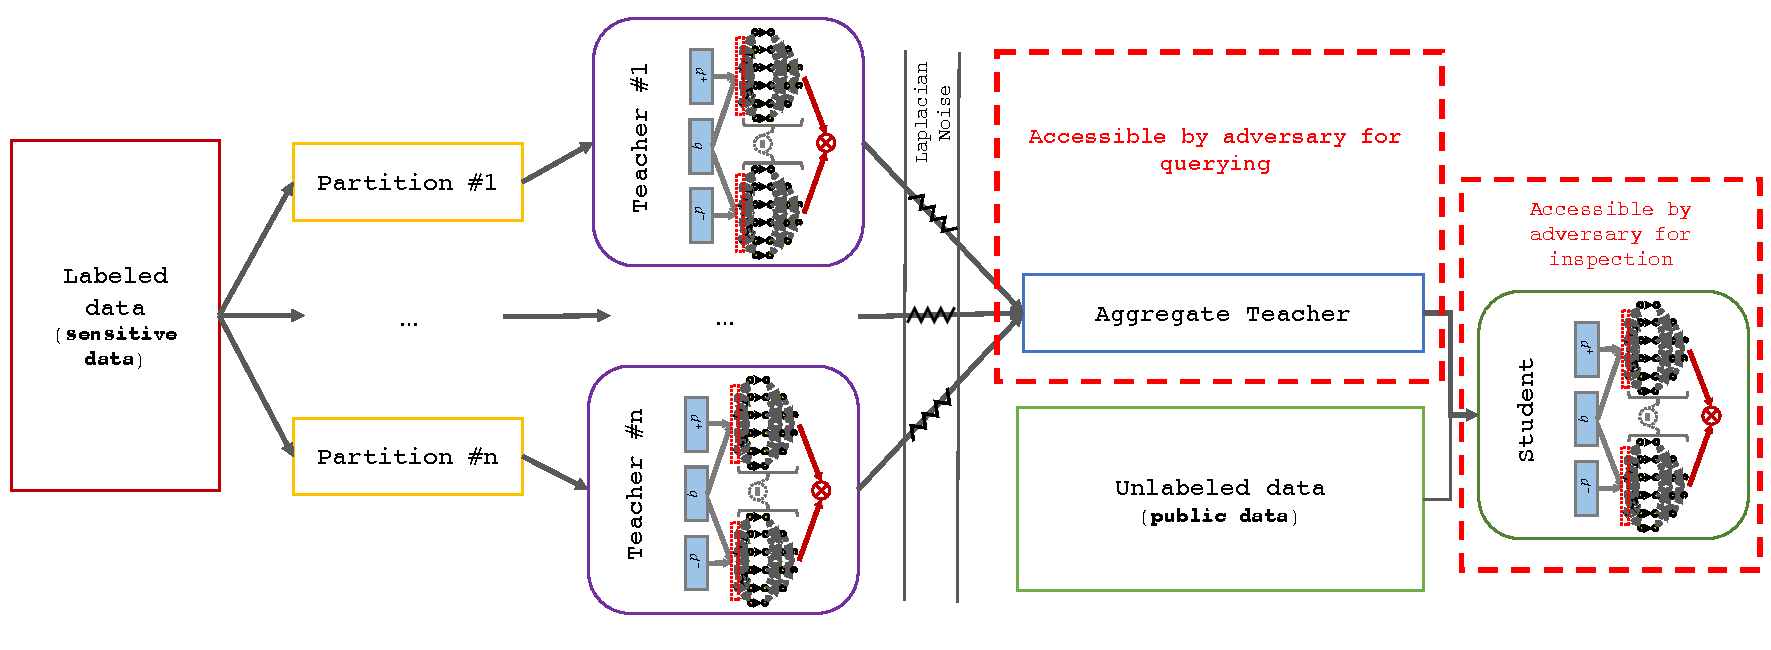
\includegraphics[height=5.5cm]{03-part-02/chapter-04/figs_and_tables/fig_privacy_preserving_ranker_model.pdf}%
    \caption{\label{fig:pp_model} Privacy preserving annotator/model sharing, proposed by~\citet{Papernot:2017}.}
\end{figure}

The general schema of the PATE is illustrated in Figure~\ref{fig:pp_model}. First, the sensitive training data is divided into $n$ partitions. Then, on each partition, an independent neural network model is trained as a teacher.  Once all the teachers are trained, an aggregation step is done using majority voting to generate a single global prediction.  
Laplacian noise is injected into the output of the prediction of each teacher before aggregation. The introduction of this noise is what protects privacy because it obfuscates the vulnerable cases, where teachers disagree. 

The aggregated teacher can be considered as a deferentially private API to which we can submit the input and it then returns the privacy preserving label. There are some circumstances where due to efficiency reasons the model is needed to be deployed to the user device~\cite{Abadi:2016}. To be able to generate a shareable model where the privacy of the training data is preserved, \citet{Papernot:2017} train an additional model called the student model. The student model has access to unlabeled public data during training. The unlabeled public data is annotated using the aggregated teacher to transfer knowledge from teachers to student model in a privacy preserving fashion. 
This way, if the adversary tries to recover the training data by inspecting the parameters of the student model, in the worst case, the public training instances with privacy preserving labels from the aggregated teacher are going to be revealed.  The privacy guarantee of this approach is formally proved using differential privacy framework.

As there is no publicly available large scaled data that we can use in our experiments as the initial sensitive labeled data, we use pseudo labels as it is explained in~\ref{sec:pseudo_labeling}\footnote{Partitioning the fully supervised training data in our problem leads to very small training sets which are not big enough to train teacher networks.}. 
In our experiments, we split the training data into three partitions, each contains one million queries annotated by the BM25 method. We train three identical teacher models. Then, we use the aggregated noisy predictions from these teachers to train the student network using the knowledge distillation approach. Configurations of teacher and student networks are similar to the previous experiments, as they are presented in Table~\ref{tbl:cfg}.

We evaluate the performance in two situations: In the first one, the privacy parameter, which determines the amount of noise, is set to zero, and in the second one, the noise parameter is set to $0.05$, which guarantees a low privacy risk~\citep{Papernot:2017}.
%
We report the average performance of the teachers before noise, the performance of noisy and non-noisy aggregated teacher, and the performance of the student networks in two situations.  The results of these experiments are reported in Table~\ref{tbl_res2}.

\begin{table}[t]
\centering
\caption{\label{tbl_res2}Performance of the teachers (average) and student models with noisy and non-noisy aggregation.}
\vspace{5pt}
\begin{adjustbox}{max width=\textwidth}
\begin{tabular}{l c c c}
\toprule
 \textbf{Model} & \textbf{MAP} & \textbf{P@20} & \textbf{nDCG@20} 
\\ \midrule
{\textbf{Teachers (avg)}}
& 0.2566 & 0.3300 & 0.3836
\\ \midrule
\textbf{Non-noisy aggregated teacher} 
& 0.2380 & 0.3055 & 0.3702 
\\
\textbf{Student \small{(non-noisy aggregation)}} 
& 0.2337 & 0.3192 & 0.3717
\\ \midrule 
\textbf{Noisy aggregated teacher} 
& 0.2110 & 0.2868 & 0.3407 
\\
\textbf{Student \small{(noisy aggregation)}} 
& 0.2255 & 0.2984 & 0.3559 
\\ \bottomrule
\end{tabular}
\end{adjustbox}
\end{table}

Results in Table~\ref{tbl_res2} suggest that using the noisy aggregation of multiple teachers as the supervision signal, we can train a neural ranker with an acceptable performance.
%
Compared to the single teacher setup in Section~\ref{sec:mimic_learning_to_rank}, the performance of the student network is not as good as the average performance of teachers. Although the student network performs better than the teacher in the noisy aggregation setup. This is more or less the case for a student together with a non-noisy aggregated teacher.
% 
We believe drops in the performance on the student networks compared to the results in Section~\ref{sec:mimic_learning_to_rank} are not just due to partitioning, noise, and aggregation. This is also the effect of the change in the amount of training data for the teachers in our experiments. We speculate that in the case of having enough training data in each partition for each teacher, their prediction will be more determined and we will have less disagreement in the aggregation phase and consequently, we will get better signals for training the student model.


